\documentclass[11pt]{exam}

\usepackage{amsmath, amssymb, multicol}
\usepackage{graphicx}
\usepackage{textcomp}
\usepackage{chessboard}
\usepackage{tikz}

\def\d{\displaystyle}
\def\b{\mathbf}
\def\R{\mathbf{R}}
\def\Z{\mathbf{Z}}
\def\st{~:~}
\def\bar{\overline}
\def\inv{^{-1}}


\newcommand{\vtx}[2]{node[fill,circle,inner sep = 0 pt, minimum size=4 pt,label=#1:#2]{}}
\newcommand{\va}[1]{\vtx{above}{#1}}
\newcommand{\vb}[1]{\vtx{below}{#1}}
\newcommand{\vr}[1]{\vtx{right}{#1}}
\newcommand{\vl}[1]{\vtx{left}{#1}}
\renewcommand{\v}{\vtx{above}{}}


%\pointname{pts}
\pointsinmargin
\marginpointname{pts}
\addpoints
\pagestyle{head}
%\printanswers

\firstpageheader{Math 228}{\bf Game of Counting}{Monday, November 27}


\begin{document}

%space for name
%\noindent {\large\bf Name:} \underline{\hspace{2.5in}}
%\vskip 1em

\noindent The two richest families in Westeros have decided to enter into an alliance by marriage.  The first family has 10 sons, the second has 10 daughters.  The ages of the kids in the two families match up.   To avoid impropriety, the families insist that each child must marry someone either their own age, or someone one position younger or older.  In fact, the graph representing agreeable marriages looks like this:

\begin{center}
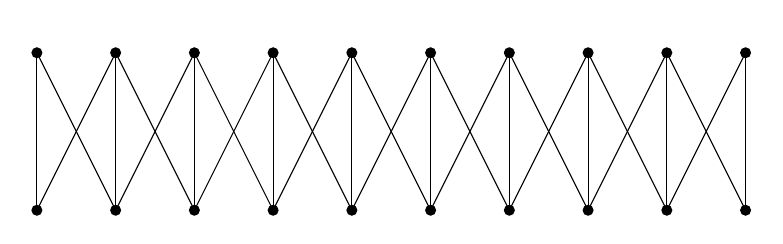
\begin{tikzpicture}
\foreach \x in {0,...,9} {
 \coordinate (a\x) at (\x,0);
 \coordinate (b\x) at (\x,2);
 \draw (a\x) \v -- (b\x) \v;
 }
\draw (a0) -- (b1) -- (a2) -- (b3) -- (a4) -- (b5) -- (a6) -- (b7) -- (a8) -- (b9);
\draw (b0) -- (a1) -- (b2) -- (a3) -- (b4) -- (a5) -- (b6) -- (a7) -- (b8) -- (a9);

\end{tikzpicture}
\end{center}

The question: how many different acceptable marriage arrangements which marry off all 20 children are possible?  Assume that polygamy is not allowed.

\begin{questions}
\question Could two brothers adjacent in age both marry girls older than them?  Explain.  Given this, what will acceptable marriage arrangements of all 20 children ``look'' like?
\begin{solution}
Call the boys $b_1, b_2, \ldots, b_{10}$ and the girls $g_1, g_2, \ldots, g_{10}$, arranged in order of age.  Say, for the sake of contradiction, that $b_k$ and $b_{k+1}$ both marry girls older than themselves.  We can say exactly who they marry: $b_k$ marries $g_{k+1}$ and $b_{k+1}$ marries $g_{k+2}$.  Who then will $b_{k+2}$ marry?  It will have to be $g_{k+3}$.  And $b_{k+3}$ will need to marry $g_{k+4}$.  In fact, we would have that for any $n$, $b_n$ will marry $g_{n+1}$.  But this is impossible because it would leave $g_1$ unmarried (there is no $b_{0}$) and $b_{10}$ unmarried (there is no $g_{11}$).  Thus no two brothers adjacent in age can both marry girls older than them.

In fact, this tells us that if any boy marries a girl older than him, his next older brother \emph{must} marry a girl younger than him (the same age as his brother).  Thus any marriage arrangement will look like a collection of I's and X's, such as this:

\begin{center}
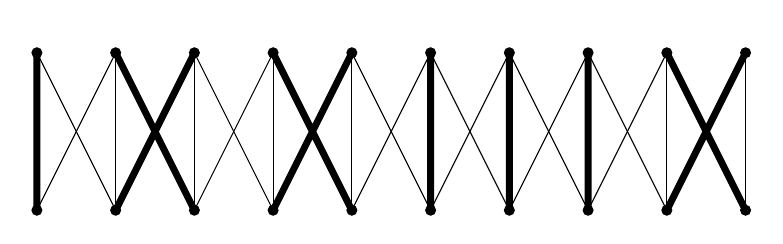
\begin{tikzpicture}
\foreach \x in {0,...,9} {
 \coordinate (a\x) at (\x,0);
 \coordinate (b\x) at (\x,2);
 \draw[thin] (a\x) \v -- (b\x) \v;
 }
\draw[thin] (a0) -- (b1) -- (a2) -- (b3) -- (a4) -- (b5) -- (a6) -- (b7) -- (a8) -- (b9);
\draw[thin] (b0) -- (a1) -- (b2) -- (a3) -- (b4) -- (a5) -- (b6) -- (a7) -- (b8) -- (a9);

\draw[line width = 2.5] (a0) -- (b0) (a1) -- (b2) (a2)-- (b1) (a3) -- (b4) (a4) -- (b3) (a5) -- (b5) (a6) -- (b6) (a7) -- (b7) (a8) -- (b9) (a9) -- (b8);
\end{tikzpicture}
\end{center}
\end{solution}
\vfill

\question How many marriage arrangements are possible if we insist that exactly 6 boys marry girls \underline{not} their own age? Hint: think about what such an arrangement would look like.  How is this like counting bit-strings?

\begin{solution}
Since such an arrangement would result in 3 X's and 4 I's, and any arrangement of 3 X's and 4 I's corresponds to exactly one marriage arrangement, we just need to count the number of strings of 7 symbols 3 of which are I's.  There are ${7 \choose 3}$ such strings.
\end{solution}


\vfill

\question Generalize the previous answer to find the number of arrangements where $2n$ boys marry a girl not their age, and use these to find total number of marriage arrangements.

\begin{solution}
We could insist that there are 0 boys who marry girls not their own age, or 2, or 4, or 6, or 8 or all 10.  Note that it would be impossible for an odd number of boys to marry girls not their own age, since these boys need to come in ``X'' creating pairs.  Adding up the number of ways each of these can happen we get
\[{10 \choose 0} + {9 \choose 1} + {8 \choose 2} + {7 \choose 3} + {6 \choose 4} + {5 \choose 5} = 1 + 9 + 28 + 35 + 15 + 1 = 89\]
Note that the ${8 \choose 2}$ (for example) comes from the number of ways in which $4$ boys could marry girls not their own age, as we need to have exactly two X's and 6 I's in such an arrangement; so we ask how many strings of 8 symbols contain exactly 2 X's?
\end{solution}



\vfill

\newpage

\question How do you know you are correct?  Try counting in a different way.  Look at smaller family sizes and get a sequence.  In other words, keeping the same sort of graph (each person connected to the three people of opposite gender closest in age), let $M_n$ be the number of marriage arrangements possible with $n$ boys and $n$ girls.  Find the sequence $M_1, M_2, M_3,\ldots$.

\begin{solution}
By inspection, we have $M_1 = 1$, $M_2 = 2$, $M_3 = 3$, and $M_4 = 5$.  In fact, it appears that $M_5 = 8$.  Could these really be the Fibonacci numbers?  To decide, we need to check that the recursive definition for $M_n$ is indeed the Fibonacci recurrence: $F_n = F_{n-1} + F_{n-2}$.

\end{solution}

\vfill

\question Give a recurrence relation for $M_n$.  Explain why you are correct.

\begin{solution}
$M_n = M_{n-1} + M_{n-2}$.  Here is why: suppose you wanted to count the number of arrangements with $n$ boys and $n$ girls.  Who could the youngest boy marry?  He could marry the youngest girl.  Remove these two from the graph and you are left with the graph for $n-1$ boys and girls, and there are $M_{n-1}$ marriage arrangements for them.  On the other hand, the youngest boy could marry the second-youngest girl.  In this case, the second youngest boy must marry the youngest girl.  Remove these 4 vertices from the graph and you are left with $n-2$ boys and girls, who can be married off in $M_{n-2}$ ways.  Since these are the only two options for the youngest boy, we have now included every possible marriage arrangement of the $n$ boys and girls.
\end{solution}



\vfill




\end{questions}

\end{document}
